% The original template for ICIP-2000 paper; to be used with:
%          spconf.sty  - ICASSP/ICIP LaTeX style file, and
%          IEEEbib.bst - IEEE bibliography style file.
% --------------------------------------------------------------------------
\documentclass{article}
\usepackage{spconf,amsmath,epsfig,url}

% Example definitions.
% --------------------
\def\x{{\mathbf x}}
\def\L{{\cal L}}

% Title.
% ------
\title{stockPricePrediction}
%
% Single address.
% ---------------
\name{Student A}
\address{Department of Computer Engineering\\ Chulalongkorn Univerisy\\ Bangkok, Thailand}

% For example:
% ------------
%\address{School\\
%		 Department\\
%		 Address}
%
% Two addresses (uncomment and modify for two-address case).
% ----------------------------------------------------------
%\twoauthors
%  {A. Author-one, B. Author-two\sthanks{Thanks to XYZ agency for funding.}}
%		 {School A-B\\
%		 Department A-B\\
%		 Address A-B}
%  {C. Author-three, D. Author-four\sthanks{The fourth author performed the work
%		 while at ...}}
%		 {School C-D\\
%		 Department C-D\\
%		 Address C-D}
%
\begin{document}
%\ninept
%
\maketitle
%
\begin{abstract}
Predicting a stock price is a very challenge task.It requires high accuracy go together with high flexibility, and the main result.  The abstract has to be
self-contained and readable for a person in the general area. You
should write the abstract last.
\end{abstract}

\section{Introduction}\label{sec:intro}

\subsection{Motivation}

Nowaday, we can see many of securities company provide a software that help customers to plan their investment strategy.
the software is also known as EA (Expert Advisor) , this brings our team curiosity.Does the EA really work? Our target is to analyze the models and to find out which model is the most practical in the stock market.

\subsection{Previous Work}

Before our experiment , we tried some basic models that base on pure dataset and found that the test score is not good as we expected.After that , our team tried to add some useful features , such as moving average to the dataset but , the test score of our new model stills not good as we expected.

\subsection{What We Are Going to Do}

Our next milestone is to generate the model that relate with time-series data.After our previous work,We found that we did not deal with noise in the dataset.The noise can be generated by trading psychology or news.So, we will focus on these noises too.

\subsection{Organization of the Paper}

In Section~\ref{sec:background} we provide the background on the investment and basic time-series analysis.

\subsection{General Comments}

\begin{itemize}
\item You do not have to follow the exact subsection titles in this section
or the others. It is just to help you get started.  Alternatively, and
what I usually do to save space, is to use paragraph titles instead of
subsections, as in

{\bf Organization of the paper.} Blabla.

\item It is generally a good idea to break sections into smaller units for
readability and since it helps you to structure the story.

\item Also, the following section titles should be adapted to more precisely
reflect what you do.

\item It is helpful to start each of the following sections with a very
short summary of what the reader can expect in the section. Nothing
more awkward as when the story starts and one does not know what the
direction is or the goal.

\item Make sure you define each acronym you use, no matter how convinced you are
the reader knows it.

\item Always spell-check before you submit (to me in this case).

\item Be picky. When writing a paper you should always strive for very
high quality. Many people may read it and the quality makes a big difference.

\item Books helping you to write better: \cite{Higham:98} and \cite{Strunk:00}.

\item Conversion to pdf (latex users only): 

dvips ... -Ppdf -G0 ....
\end{itemize}


\section{Necessary Background}
\label{sec:background}


We divide topics in this part into 4 parts are as follows :\\
1. knowledge about investment\\
2. What is time-series\\
3. The model that we decide to use\\
4. Details between training our model


\subsection{Investment}
Everyday,there are many investors trade stocks with each other.The buyers have the money but, they would like to hold stocks instead of money , on the other hand , the sellers already have stocks but, they would like to sell their stocks and keep money instead.The market is the place that allow investors to trade with each other.Trading transaction will be happened when buyer and seller make a deal.
Price mechanism is also created by this event too.

\subsection{Basic time-series Analysis}
\begin{itemize}
\item What is time-series?\\A time series is a sequence of data that ordered by time.Stock price at time N will 
effect to stock price at time N+1
\item Stocks data is also a time series that has seasonality (each stock has opportunity day itself).
\end{itemize}


\subsection{ARIMA Model}
ARIMA, short for "Auto Regressive Integrated Moving Average", is one of the machine learning model for manipulate with time series data.The ARIMA model is divided into 3 terms :\\p is the order of AR term\\q is the order of MA term\\d is the number of differencing required to make the time series stationary.


\subsection{Model training}
\begin{itemize}
\item Explain
\end{itemize}

\section{Your Proposed Method}\label{sec:yourmethod}

Here you explain what you did, again first starting with a brief overview.
Structure it as suitable. 

{\bf Note: You have to:}
\begin{itemize}
\item Explain all steps you performed so that another person can re-produce your experiments as close as possible
\item This can be exactly like the paper you try to replicate. However, you should try to explain it it your own words. Most paper has space constraints and left out many details and hyperparameter choices. Describe what you use.
\end{itemize}


\section{Experimental Results}
\label{sec:exp}

Here you evaluate your work using experiments.  You start again with a very short summary, and then you
give the experimental setup. 

{\bf Note: You have to:}
\begin{itemize}
\item explain the metrics. Explain the dataset.
\item very readable, attractive plots (1 column, not 2 column plots),
proper font size
\item every plot answers a question, which you pose and extract the
answer from the plot in its discussion
\item analyze the errors. Which errors are hard and why (rare class, noisy feature)? Give example errors and why some model can handle some kind of error better than the others.
\end{itemize}

\section{Conclusions}
\label{sec:conclusion}

Here you need to summarize what you did and why this is important.  DO
NOT TAKE THE ABSTRACT and put it in the past tense. Instead, try to
highlight important results and their (potential) impact on your
problem. Say something about what you could do next and what is on
your wish list of improvements to your present method.


\section{Citing}
\label{sec:cite}

You can reference a paper by creating a key-value pair in conference.bib (at the bottom of the file, see example file). The format of the citation information follows bibtex format. Most journal websites or google scholar have a section where you can easily copy and paste the bibtex of the paper (see Figure \ref{fig:bibtex}). To cite, just use $\backslash cite\{key\}$. 

\begin{figure}
  \centering
  \centerline{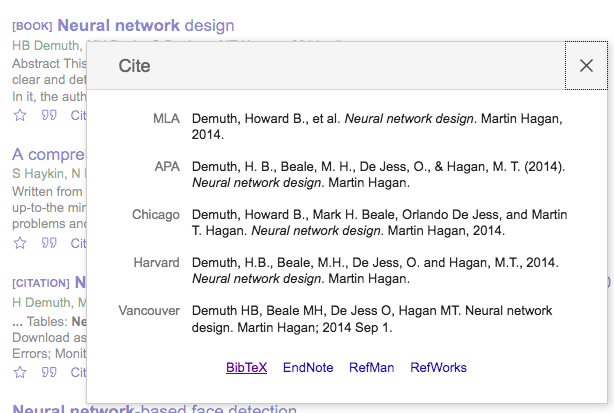
\includegraphics[width=0.45\textwidth]{bibtex.png}}
  \caption{Example of how to find the bibtex on Google Scholar. Click on the quotation marks, then select bibtex.}
  \label{fig:bibtex}
\end{figure}

\section{Latex basics}
\label{sec:latex}

By this point, you probably notice that latex is quite simple and intuitive. If you are curious about more, try consulting \url{http://www.stat.pitt.edu/stoffer/freetex/latex%20basics.pdf}.

For a short version of things to know, this template already cover the basics. Note how you can reference a section, figure, or table by using $\backslash ref\{\}$, refering to some $\backslash label\{\}$ you define elsewhere in the document.

Finally, this is how you define a table.

\section{Latex editor}

There are many latex editor. One is MikTEX. There are also online tools called sharelatex \footnote{\url{https://www.sharelatex.com/}}. I recommend using this service since it require no installation. You can try for free but in order to use the more advance features (online collaboration and version control) you need to pay for its service. I have a paid subscription. If you want to use the online collaboration feature, contact me and I will host the project for your group.

\begin{table}
\centering
\begin{tabular}{|l|c|c|c|c|} % this defines how many columns and indentation of each column
 \hline % creates a horizontal line
First & 2nd & 3rd & 4th \\ %columns are separated by & and newline is \\
 \hline
 Phones & 28 & 48 & 38 \\
 Tones & n/a & n/a & n/a \\
 Graphemes & 27 & 57 & 28 \\
 Amount & 3 & 3 & 3 \\
 Wideband & yes & yes & yes \\
 Vocab & 3.7k & 7.3k & 5.4k \\
 Word count & 33k & 25k & 27k \\
 Speakers & 358 & 362 & 371 \\
 Web data amount & 38.0M & 6.4M & 16.2M \\
 \hline
\end{tabular}
\caption{Some table}
\label{tab:table}
\end{table}

% References should be produced using the bibtex program from suitable
% BiBTeX files (here: bibl_conf). The IEEEbib.bst bibliography
% style file from IEEE produces unsorted bibliography list.
% -------------------------------------------------------------------------
\bibliographystyle{IEEEbib}
\bibliography{conference}

\end{document}

